\begin{frame}\begin{center}
		\LARGE\textit{Marginal Effect of Treatment}
\end{center}\end{frame}
%-------------------------------------------------------------------------------
%-------------------------------------------------------------------------------
\begin{frame}\textbf{Marginal Benefit of Treatment}
	\begin{align*}
		B^{MTE}(x, u_D) = E [Y_1 - Y_0 \mid X = x,  U_D = u_D]
	\end{align*}	
	\textbf{Intuition:} Mean gross return to treatment for persons at
	quantile \(u_D\) of the first-stage unobservable \(V\) or a willingness to pay for individuals at the margin of indifference.
\end{frame}
%-------------------------------------------------------------------------------
%-------------------------------------------------------------------------------
\begin{frame}
	\begin{figure}\caption{Margin of Indifference}
		\scalebox{0.35}{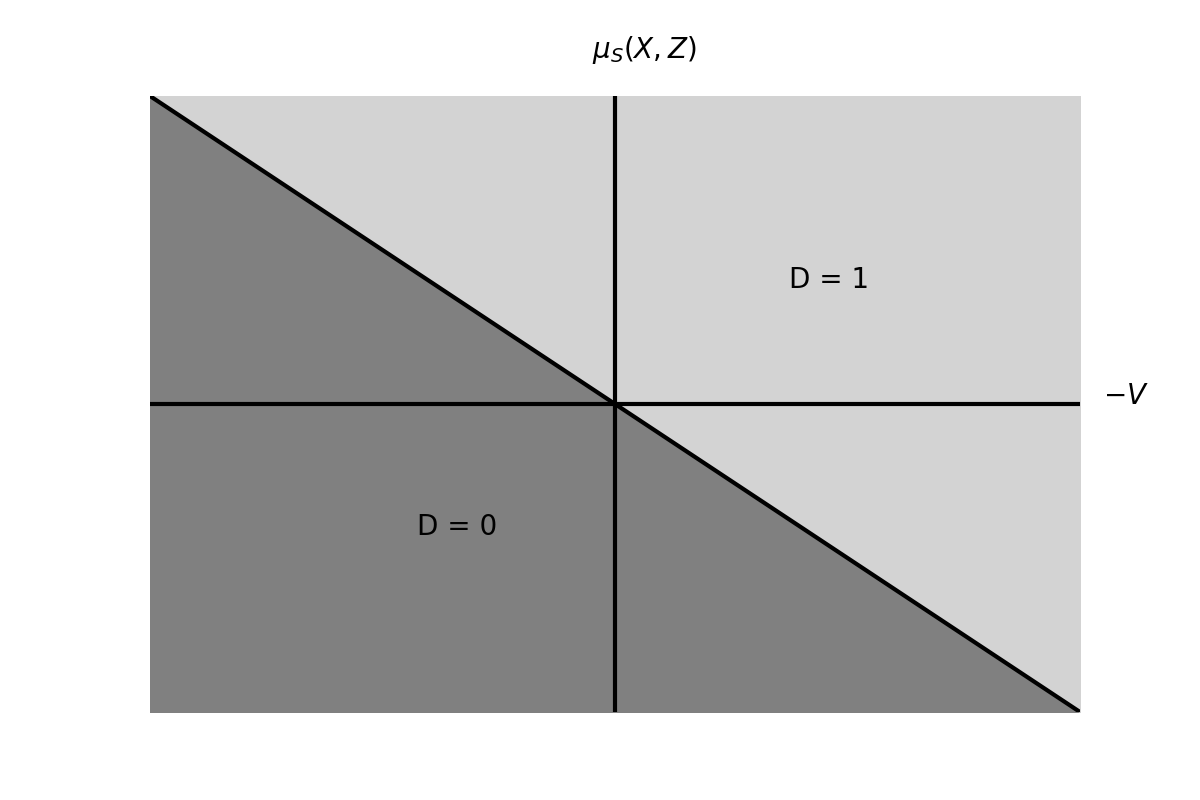
\includegraphics{fig-margin-indifference}}
	\end{figure}
\end{frame}
%-------------------------------------------------------------------------------
%-------------------------------------------------------------------------------
\begin{frame}	
	\begin{figure}\caption{Marginal Benefit of Treatment}
		\scalebox{0.35}{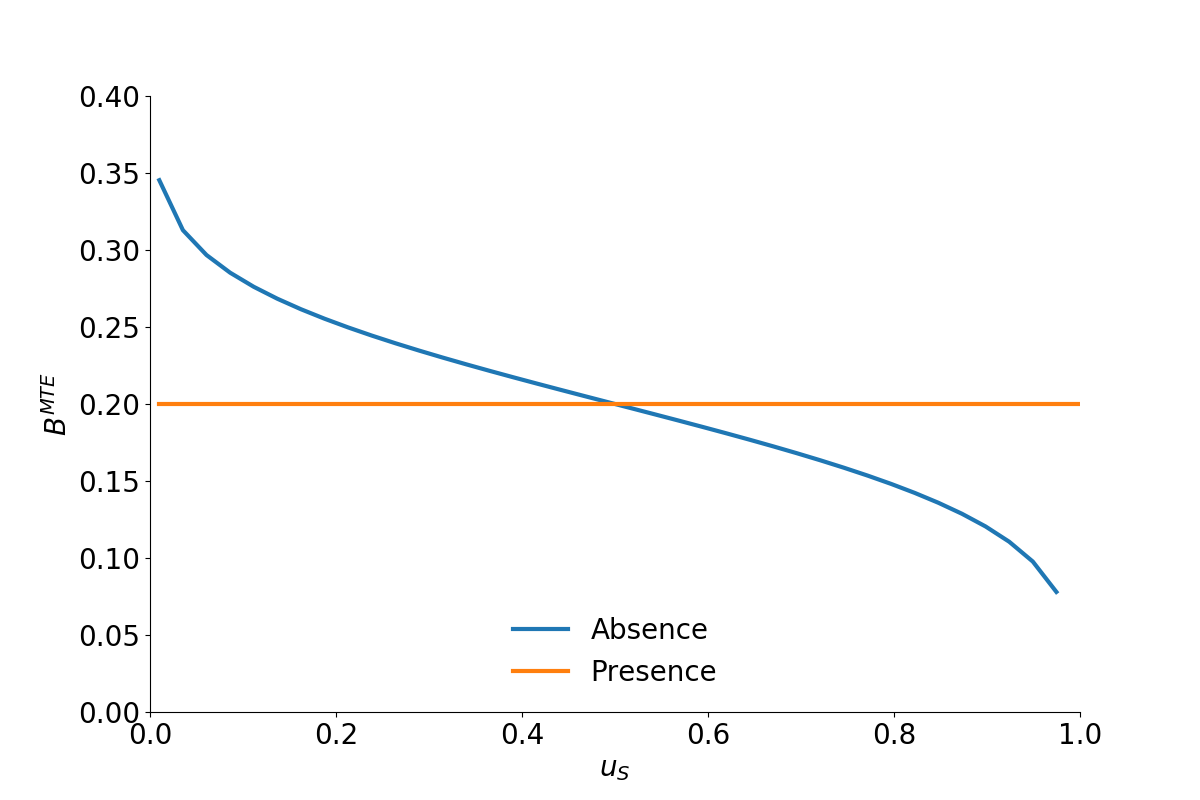
\includegraphics{fig-eh-marginal-effect}}
	\end{figure}
\end{frame}
%-------------------------------------------------------------------------------
%-------------------------------------------------------------------------------
\begin{frame}
	\textbf{Effects of Treatment as Weighted Averages}
	Parameter \(\Delta_j\), can be written as a weighted average of the
	\(B^{MTE}(x, u_D)\).
	\begin{align*}
		\Delta_j(x) = \int_0^1 B^{MTE}(x, u_D) \omega^j(x, u_D) du_D,
	\end{align*}
	where the weights \(\omega^j(x, u_D)\) are specific to parameter \(j\)
	and integrate to one.
\end{frame}
%-------------------------------------------------------------------------------
%-------------------------------------------------------------------------------
\begin{frame}
	\textbf{Weights}	
	\begin{align*}
		\omega^{ATE}(x, u_D) & = 1 \\
		\omega^{TT}(x, u_D) & = \frac{1 - F_{P\mid X=x}(u_D)}{E[P \mid X = x]}\\
		\omega^{TUT}(x, u_D) & = \frac{F_{P\mid X=x}(u_D)}{E[1 - P \mid X = x]}
	\end{align*}	
\end{frame}
%-------------------------------------------------------------------------------
%-------------------------------------------------------------------------------
\begin{frame}
	\begin{figure}\caption{Effects of Treatment as Weighted Averages}
		\scalebox{0.6}{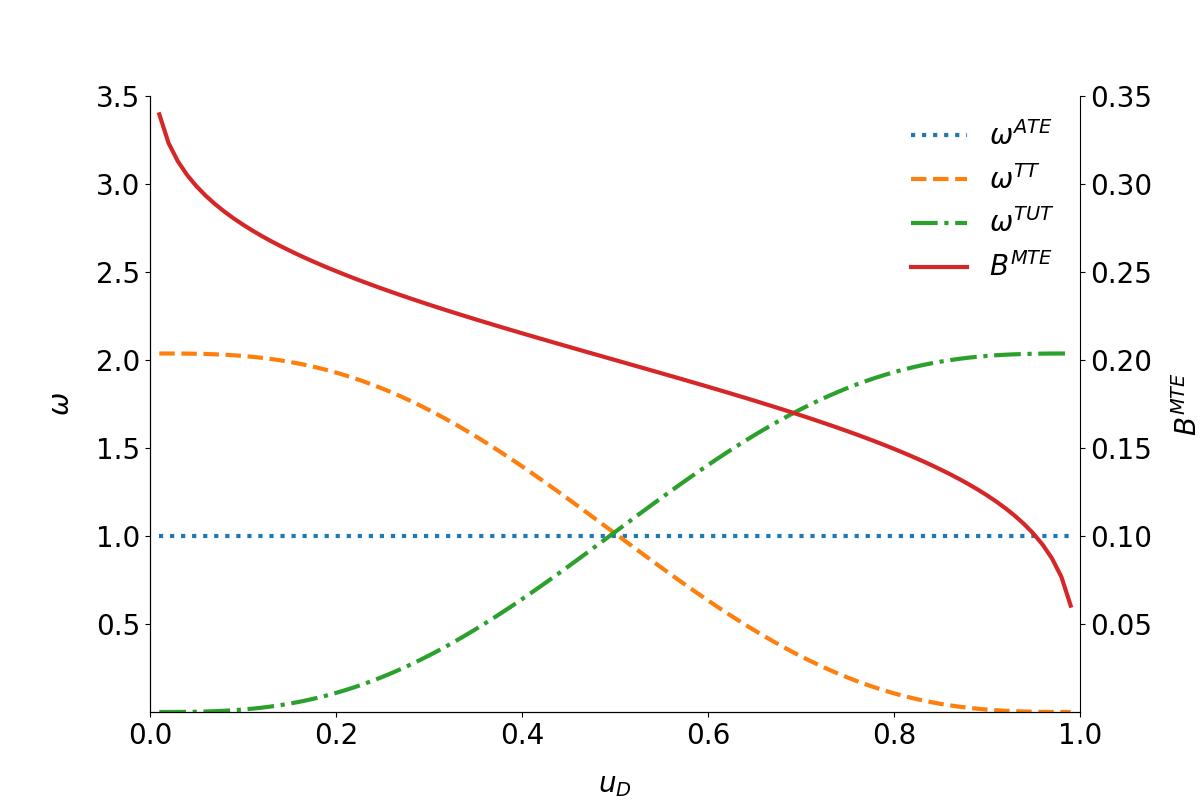
\includegraphics{fig-weights-marginal-effect}}
	\end{figure}
\end{frame}
